\documentclass{article}
\usepackage[paper=letterpaper,margin=2cm]{geometry}
\usepackage[utf8]{inputenc}
\usepackage[russian]{babel}
\usepackage[]{graphicx}
\usepackage[usenames]{color}
\usepackage{colortbl}
\usepackage{geometry}
\usepackage{xcolor}
\usepackage{hyperref}
\usepackage{../../lib/latex/listings-rust}
\usepackage{fontspec}
\setmonofont{JetBrains Mono}[Contextuals=Alternate,Ligatures = TeX,]
\usepackage{listings}
\usepackage{keycommand}
\usepackage{caption}

\setmainfont[
  Ligatures=TeX,
  Extension=.otf,
  BoldFont=cmunbx,
  ItalicFont=cmunti,
  BoldItalicFont=cmunbi,
]{cmunrm}
\setsansfont[
  Ligatures=TeX,
  Extension=.otf,
  BoldFont=cmunsx,
  ItalicFont=cmunsi,
]{cmunss}

\geometry{
  a4paper,
  top=25mm,
  right=30mm,
  bottom=25mm,
  left=30mm
}

\hypersetup{
  colorlinks=true,
  linkcolor=blue!50!red,
  urlcolor=blue!70!black
}

\captionsetup[lstlisting]{
  font={tt},
}

% based on Atom One Light
\lstset{
  language=Java,
  frame=single,
  basicstyle=\ttfamily\color[HTML]{383a42},
  columns=fullflexible,
  breaklines=true,
  numbers=left,
  frame=tab,
  postbreak=\mbox{\textcolor{red}{$\hookrightarrow$}\space},
  extendedchars=false,
  showspaces=false,
  showstringspaces=false,
  identifierstyle=\ttfamily\color[HTML]{4078f2},
  commentstyle=\color[HTML]{a0a1a7},
  stringstyle=\color[HTML]{50a14f},
  keywordstyle=\color[HTML]{a626a4},
  numberstyle=\ttfamily\color[HTML]{2c91af},
  rulecolor=\color[HTML]{383a42}
}

\lstdefinelanguage{XML}
{
  morestring=[b]",
  morestring=[s]{>}{<},
  morecomment=[s]{<?}{?>},
}

\newcommand{\code}[1]{
  \lstset{title=#1}
  \lstinputlisting{#1}
}
\newkeycommand{\itmo}[variant=aboba, labn=aboba, discipline=aboba, group=aboba, student=aboba,teacher=aboba, year=2022]{
  \begin{titlepage}
    \begin{center}
      \section*{
        Федеральное государственное автономное образовательное учреждение\\ высшего образования\\
        «Национальный исследовательский университет ИТМО»\\
        Факультет Программной Инженерии и Компьютерной Техники \\
       }
      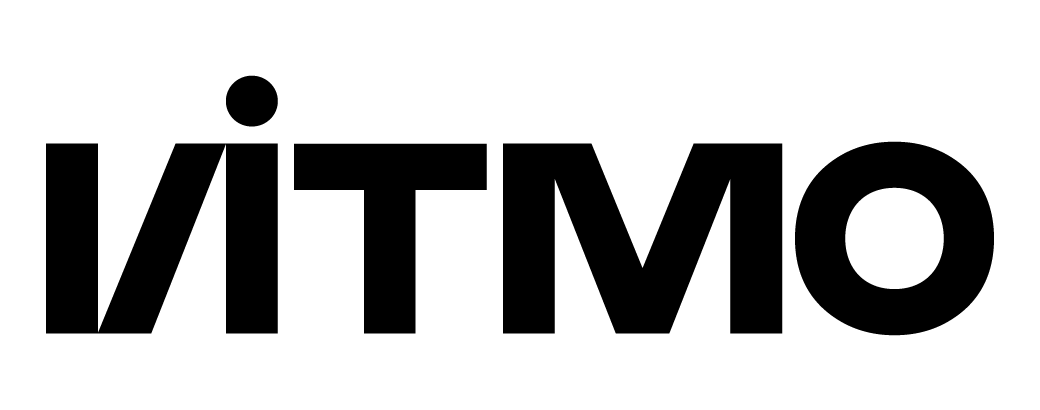
\includegraphics[scale=0.2]{../../lib/img/itmo.png}
    \end{center}

    \vspace{4cm}

    \begin{center}
      \large \textbf{Вариант \textnumero \commandkey{variant}}\\
      \textbf{Лабораторная работа \textnumero \commandkey{labn}}\\
      по дисциплине\\
      \textbf{\commandkey{discipline}}
    \end{center}

    \vspace*{\fill}

    \begin{flushright}
      Выполнил Студент группы \commandkey{group}\\
      \textbf{\commandkey{student}}\\
      Преподаватель: \\
      \textbf{\commandkey{teacher}}\\
    \end{flushright}

    \vspace{1cm}

    \begin{center}
      г. Санкт-Петербург\\
      \commandkey{year}г.
    \end{center}

    \thispagestyle{empty}
  \end{titlepage}
}


\begin{document}

\itmo[
  variant=15677557,
  labn=3,
  discipline=Программирование,
  group=P3115,
  student=Владимир Мацюк,
  teacher=Сорокин Роман Борисович
]

\tableofcontents

\section{Текст задания}
\subsection{Описание предметной области, по которой должна быть построена объектная модель:}

Шла генеральная репетиция пьесы Муми-папы, и горели все лампы, хотя до вечера было еще далеко. Бобрам пообещали контрамарки на премьеру, назначенную на следующий день. За это они сняли театр с мели и вывели его на глубину. Сцена, правда, все же была слегка перекошена, что было довольно неудобно.
\subsection{Программа должна удовлетворять следующим требованиям:}
\begin{enumerate}
  \item Доработанная модель должна соответствовать принципам SOLID.
  \item Программа должна содержать как минимум два интерфейса и один абстрактный класс (номенклатура должна быть согласована с преподавателем).
  \item В разработанных классах должны быть переопределены методы equals(), toString() и hashCode().
  \item Программа должна содержать как минимум один перечисляемый тип (enum).
\end{enumerate}
\subsection{Порядок выполнения работы:}
\begin{enumerate}
  \item Доработать объектную модель приложения.
  \item Перерисовать диаграмму классов в соответствии с внесёнными в модель изменениями.
  \item Согласовать с преподавателем изменения, внесённые в модель.
  \item Модифицировать программу в соответствии с внесёнными в модель изменениями.
\end{enumerate}



\section{Вывод}
Во время выполнения работы я ознакомился с ООП на языке java. Научился разрабатывать архитектуру проекта и подключать jar архивы к проекту.
\end{document}
